\documentclass[a4paper, 12pt, oneside]{report}

\usepackage[utf8]{inputenc}
\usepackage{lmodern}
\usepackage{layout}
\usepackage{emptypage}
\usepackage{fancyhdr}
%\usepackage[Conny]{fncychap}
%\usepackage{graphicx}
\usepackage{subfigure} % subfiguras
\usepackage{caption}
\usepackage{mathtools}
\usepackage{hyperref}
\usepackage[a4paper,top=3cm, bottom=3cm, inner=2.5cm, outer=2.5cm]{geometry}
\usepackage{listings}
\usepackage[spanish]{babel}
\usepackage{url}

\usepackage{titlesec}
\makeatletter
\renewcommand{\@makeschapterhead}[1]{%
%  \vspace*{50\p@}%
  \vspace*{0\p@}%
  {\parindent \z@ \raggedright
    \normalfont
    \interlinepenalty\@M
    \Huge \bfseries  #1\par \nobreak
%    \vskip 40\p@
    \vskip 15\p@
  }}
\makeatother

\renewcommand{\baselinestretch}{1.4}
\setlength{\headheight}{16pt} 

\pretolerance=1000

\chead[]{}
\rhead[]{}
\renewcommand{\headrulewidth}{0.5pt}

\pagestyle{empty}

\title{Deep-learning para detección de vehículos}
\author{Nuria Oyaga de Frutos}

\lstset{
	float=hbp,
	basicstyle=\ttfamily\small,
	columns=flexible,
	tabsize=4,
	frame=single,
	extendedchars=true,
	showspaces=false,
	showstringspaces=false,
	numbers=none,
	numberstyle=\tiny,
	breaklines=false,
	breakautoindent=true,
	captionpos=b
}

\begin{document}
%%%%%%%%%%%%%%% Portada %%%%%%%%%%%%%%%%%%%%
\begin{titlepage}
	
	\begin{center}
		\vspace*{7.7mm}
		\begin{center}
			
\includegraphics[width=0.4\linewidth]{figures/logo.jpg}
		\end{center}
		\vspace{6.5mm}
		
		\fontsize{15.5}{14}\selectfont ESCUELA TÉCNICA SUPERIOR DE INGENIERÍA DE TELECOMUNICACIÓN
		\vspace{13mm}
		
		\fontsize{14}{14}\selectfont GRADO EN INGENIERÍA EN SISTEMAS \\ AUDIOVISUALES Y MULTIMEDIA
		
		\vspace{70pt}
		
		\fontfamily{lmss}\fontsize{15.7}{14}\selectfont \textbf{TRABAJO FIN DE GRADO} 
		
		\vspace{25mm}
		\begin{huge}
			Análisis de Aprendizaje Profundo com\\ la plataforma Caffe
		\end{huge}
		
		\vspace{25mm}
		
		\begin{large}
			Autor: Nuria Oyaga de Frutos
			
			Tutor: Inmaculada Mora Jiménez
			
			Cotutor: José María Cañas Plaza
			
			\vspace{10mm}
		\end{large}
		\begin{normalsize}
			Curso académico 2016/2017		
		\end{normalsize}
		\vspace{10mm}
		
	\end{center}
	
\end{titlepage}

\pagebreak
\thispagestyle{empty}
\vspace*{12cm}

\begin{flushright}


\includegraphics[height=1.0cm]{figures/CC-BY-SA.png}

\vspace*{0.5cm}

\copyright 2017 Nuria Oyaga de Frutos

\vspace*{0.3cm}

Esta obra está distribuida bajo la licencia de 

``Reconocimiento-CompartirIgual 4.0 Internacional (CC BY-SA 4.0)''

de Creative Commons.

\vspace{0.2cm}

Para ver una copia de esta licencia, visite

http://creativecommons.org/licenses/by-sa/4.0/ o envíe

una carta a Creative Commons, 171 Second Street, Suite 300,

San Francisco, California 94105, USA.

\end{flushright}

\pagenumbering{Roman}

%%%%%%%%%%%%%%% Agradecimientos %%%%%%%%%%%%
\chapter*{Agradecimientos}

%%%%%%%%%%%%%%% Resumen %%%%%%%%%%%%%%%%%%%%
\chapter*{Resumen}

En los últimos años, la investigación para conseguir que las máquinas perciban escenas y estímulos visuales con la robustez y rapidez que lo hacen los humanos, ha sido altamente desarrollada. En este aspecto, el campo de la Inteligencia Artificial, y en concreto nuevos esquemas de aprendizaje máquina como el aprendizaje profundo (\textit{Deep Learning}) con redes neuronales convolucionales, han experimentado un claro avance, permitiendo por ejemplo la identificación robusta de personas o la detección fiable de vehículos. A diferencia de otros, este aprendizaje no requiere de una etapa externa de extracción de características, pues la extracción se realiza en la propia red. Este trabajo analiza las redes neuronales convolucionales mediante el uso de la plataforma Caffe, que permite el entrenamiento de estas redes y facilita la implementación en aplicaciones propias.\\

En visión artificial, las redes neuronales pueden ser utilizadas para la resolución de dos problemas. Por un lado, pueden clasificar el contenido de una imagen en una categoría de entre un conjunto de clases indicadas durante el aprendizaje. Por otro lado, pueden detectar estímulos dentro de la imagen, obteniendo como salida un conjunto de cajas delimitadoras que indiquen la presencia de determinados estímulos.\\

En este trabajo se ha construido un componente en Python que clasifica números manuscritos utilizando una red neuronal de Caffe. También se ha estudiado el efecto que entrenar la red con diferentes bases de datos tiene sobre las prestaciones del clasificador. Se ha utilizado la base de datos MNIST, compuesta por imágenes de dígitos manuscritos. A esta base de datos se le ha aplicado un preprocesamiento para lograr una red más robusta. En concreto, se han considerado transformaciones de escalado, rotación, traslación y contaminación con ruido aditivo. Posteriormente, se ha aplicado un filtro de bordes de Sobel para diseñar una red que premita resolver el problema independientemente de la procedencia de las imágenes (base de datos MNIST, imágenes captadas con una cámara). Adicionalmente, tambien se ha explorado la detección de estímulos interesantes con redes neuronales de Caffe.

%%%%%%%%%%%%%%% Índices %%%%%%%%%%%%%%%%%%%%
\renewcommand{\tablename}{Tabla}
\renewcommand{\listtablename}{Índice de tablas}
\tableofcontents
\listoffigures % Í­ndice de figuras
%\listoftables % Í­ndice de tablas
\cleardoublepage

%%%%%%%%%%%%%%% Capí­tulos %%%%%%%%%%%%%%%%%%
\pagestyle{fancy}
\pagenumbering{arabic}
\setlength{\parindent}{6mm}

\lhead[]{CAPÍTULO \thechapter. INTRODUCCIÓN}
\chapter{Introducción y objetivos}\label{cap.introduccion}
El objetivo general de este trabajo se sitúa en  entender el funcionamiento del aprendizaje profundo con redes neuronales, utilizando para ello una de las plataformas existentes para el desarrollo de las mismas, Caffe.\\

En este capítulo se situará el trabajo en el marco existente en la actualidad, explicando de manera genérica en qué consiste el aprendizaje profundo, el por qué del uso de una determinada plataforma y los problemas que es posible abordar con esta técnica. Además, se expondrán los objetivos concretos de este proyecto, la metodología empleada para alcanzarlos y un pequeño resumen de cómo se ha estructurado el trabajo.

\section{Contexto y motivación}

Desde que los primeros ordenadores fueron programados, el ser humano se ha planteado la posibilidad de conseguir que estas máquinas adquieran inteligencia, logrando que realicen tareas propias de las personas. Ejemplos de estas tareas son automatizar el trabajo de rutina, entender el habla o las imágenes, hacer diagnósticos en medicina y apoyar la investigación científica básica. Hoy en día, la \acrfull{ia}~\cite{Goodfellow-et-al-2016}, como se denomina al campo que desarrolla estas tareas, cada vez adquiere más presencia, con un alto potencial por sus muchas aplicaciones prácticas y temas de investigación activos.\\

En los orígenes de la \acrshort{ia} se abordaron y resolvieron problemas que no son de resolución inmediata para los seres humanos, pero relativamente sencillos para los ordenadores, problemas que pueden describirse mediante una lista de reglas formales. Una meta actual, aún más ambiciosa, consiste en resolver tareas que son fáciles de realizar para las personas pero difíciles de describir formalmente.Se trata de problemas que son resueltos de manera rápida e intuitiva por el ser humano como, por ejemplo, el reconocimiento visual de las personas.\\

La \acrshort{ia} abarca varios campos y en este trabajo el foco estará puesto sobre la \acrfull{va}. La \acrshort{va} trata de analizar y procesar imágenes del mundo real de tal manera que un ordenador pueda establecer conclusiones sobre las mismas. La idea básica es tratar de trasladar a una máquina la forma en que el ser usa sus ojos y su cerebro para comprender el mundo que le rodea, permitiendo a las mismas tomar decisiones y actuar según la situación. Para lograr el aprendizaje de las máquinas es necesario aplicar conocimientos de distintos campos como la geometría, la estadística, la física y otras disciplinas.\\

Para conseguir materializar el concepto de la \acrshort{va} se hace uso de las Redes Neuronales Artificiales (RNA). Estas redes están compuestas por capas de neuronas interconectadas que tratan de imitar el comportamiento de las mismas en el cerebro del ser humano. La neurona biológica, consta de un cuerpo celular (soma) del que surge un denso árbol de ramificaciones (dendritas) y una fibra tubular (axón). Esta estructura se asemeja a un procesador de información simple formado por un canal de entrada, similar a las dentritas, un procesador, cuya función se asemeja a la del soma, y un canal de salida, equiparable al axón~\cite{rna}. Además, entre las neuronas biológicas se establecen una serie de conexiones unidireccionales, conocidas como sinapsis, que son emuladas en el sistema artificial por el conjunto de pesos. En la Figura~\ref{fig.rna} se muestra la similitud entre ambos tipos de neuronas. Una vez entendida la unidad de proceso, se puede definir una \acrshort{rna} como la conexión de este elemento de diferentes formas, dando lugar a diferentes tipos de redes. Para este trabajo tiene interés la red multicapa, que se compone de dos o más capas de neuronas que están conectadas entre ellas, realizando un procesado no lineal de los datos que se presentan a la entrada.\\

\begin{figure}[H]
	\begin{center}
		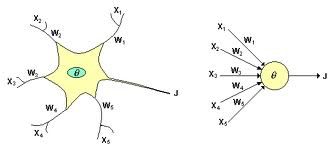
\includegraphics[width=0.7\textwidth]{figures/rna.jpg}
		\caption{Comparación de neurona artificial (derecha) y biológica (izquierda). Imagen obtenida de~\cite{rna}.}
		\label{fig.rna}
	\end{center}
\end{figure}

Tras definir el contexto general, este trabajo se centra en el Aprendizaje Profundo, situado dentro del marco de la IA, que permite obtener el conocimiento entrenando a las máquinas con ejemplos, sin necesidad de realizar una extracción de características previa, sino que es la propia red que se obtiene la encargada de ello. En la Figura~\ref{fig.aprendizaje}, se sitúa esta solución en el marco de la \acrshort{ia} y sus diferentes divisiones.

\begin{figure}[H]
	\begin{center}
		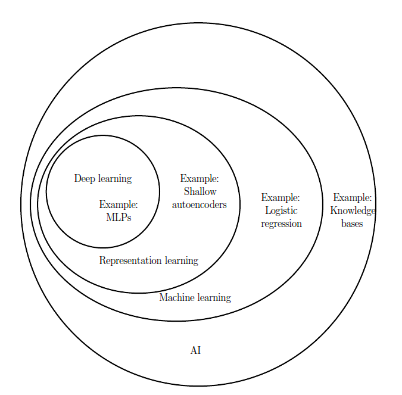
\includegraphics[width=0.6\textwidth]{figures/aprendizaje}
		\caption{Diagrama de Venn que muestra el marco de la \acrshort{ia}. Imagen obtenida de~\cite{Goodfellow-et-al-2016}.}
		\label{fig.aprendizaje}
	\end{center}
\end{figure}

En términos generales, la \acrshort{ia} contiene al Aprendizaje Máquina (\textit{Machine Learning}) definido como la capacidad de las computadoras para adquirir sus propios conocimientos, extrayendo patrones de datos sin procesar. A su vez, en el interior de la misma se sitúa el Aprendizaje de la Representación (\textit{Representation Learning}), que utiliza el aprendizaje máquina para descubrir, no sólo el mapeo de la representación a la salida, sino también la representación misma. Finalmente, en este último bloque estaría situado el Aprendizaje Profundo (\textit{Deep~Learning}), que permite a la computadora construir conceptos complejos a partir de conceptos más sencillos.\\

Dentro del Aprendizaje Profundo es posible aplicar diversas técnicas. La técnica más común y la que será empleada en este trabajo son las \acrfull{cnn}, que pretenden simular el funcionamiento del cerebro humano para establecer conclusiones sobre los datos introducidos a la misma utilizando filtros convolucionales.  La propiedad más importante del aprendizaje con redes neuronales es la capacidad de generalización, que será estimada gracias a una base de datos específica, denominada de test. Se trata de la capacidad que tiene una red de identificar una muestra que no era conocida para ella.\\

Las \acrshort{cnn} tienen una estructura especial, mostrada en la Figura~\ref{fig.cnn}. Está compuesta, generalmente, por una capa convolucional, que implementa una operación de convolución, y una capa de submuestreo o agrupación, que genera características invariantes calculando estadísticas de las activaciones de convolución a partir de un pequeño campo receptivo. Cada neurona en una capa oculta se conectará a un pequeño campo de la capa anterior, denominado campo receptivo local. En las \acrshort{cnn}, las neuronas están organizadas en múltiples capas ocultas paralelas, denominadas mapas de características, de tal manera que cada neurona en un mapa de características está conectada a un campo receptivo local. Para cada mapa de características, todas las neuronas comparten el mismo parámetro de peso que se conoce como filtro o \textit{kernel}~\cite{cnn}.

\begin{figure}[H]
	\begin{center}
		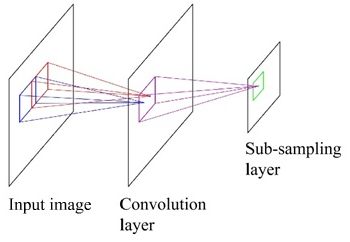
\includegraphics[width=0.4\textwidth]{figures/cnn}
		\caption{Estructura de \acrshort{cnn}. Imagen obtenida de~\cite{cnn}.}
		\label{fig.cnn}
	\end{center}
\end{figure}

En la actualidad existen múltiples disciplinas que tratan de incluir esta tecnología en su ámbito de trabajo para obtener resultados de forma más rápida y precisa. Una de las disciplinas que mas esfuerzos pone en la investigación de este campo es la medicina, cuyo principal objetivo es lograr diagnosticar y tratar, e incluso prevenir enfermedades como el cáncer. Un ejemplo de ello fue llevado a cabo por el \textit{\acrfull{bidmc}} y la Escuela de Medicina de Harvard, que consiguió el premio máximo en dos categorías del \acrfull{isbi} para la detección del cáncer de mama. El equipo, utilizando la plataforma Caffe, comenzó entrenando su máquina con cientos de diapositivas marcadas para indicar qué partes tienen células cancerosas y cuáles normales, identificando qué tipo de diapositivas eran más complicadas y alimentando el sistema con muestras más difíciles. Con este método, se obtuvo un acierto 92 por ciento y, aunque todavía no compite con los patólogos humanos, cuya precisión es el 96 por ciento, se obtiene un gran avance en este campo~\cite{2016arXiv160605718W}.\\

\begin{figure}[H]
	\begin{center}
		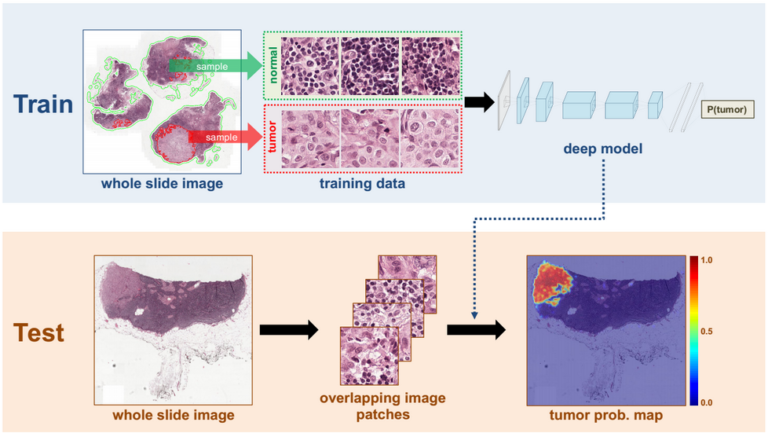
\includegraphics[width=0.6\textwidth]{figures/cancer}
		\caption{Marco utilizado para la detección del cáncer de mama. Imagen obtenida de~\cite{2016arXiv160605718W}.}
	\end{center}
\end{figure}

Un segundo ejemplo que está a la orden del día es la aplicación en la conducción autónoma. La idea de que un coche pueda manejarse en la carretera por sí mismo, sin necesidad de la existencia de un conductor que realice el trabajo, es tan llamativa que existen múltiples organizaciones que tratan de abarcar este problema. Existen tres paradigmas, mostrados en la Figura~\ref{fig.conduccion}, que permiten abarcar el problema de la conducción autónoma: (1)~el enfoque de percepción mediada, que analiza una escena entera para tomar una decisión de conducción; (2)~el enfoque de reflejo de comportamiento, que directamente mapea una imagen de entrada a una acción de conducción por un regresor; y (3)~el enfoque basado en la percepción directa para estimar la posibilidad para conducir. Este último fue desarrollado por la Universidad de Princeton se propone mapear una imagen de entrada a un pequeño número de indicadores de percepción clave, que se relacionan directamente con la disponibilidad de un estado de carretera o tráfico para la conducción. Esta representación proporciona un conjunto de descripciones compactas pero completas de la escena, permitiendo a un controlador conducir de forma autónoma.

\begin{figure}[H]
	\begin{center}
		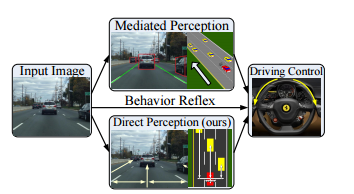
\includegraphics[width=0.6\textwidth]{figures/conduccion}
		\caption{Paradigmas de la conducción autónoma. Imagen obtenida de~\cite{2015arXiv150500256C}.}
		\label{fig.conduccion}
	\end{center}
\end{figure}

Otro ejemplo de aplicación es la traducción automática que, a pesar de haber existido durante mucho tiempo, el aprendizaje profundo consigue los mejores resultados en la traducción automática de texto e imágenes. Gracias a las \acrshort{cnn} es posible identificar las imágenes que tienen letras y dónde se situan éstas en la escena. Una vez identificadas, pueden convertirse en texto, traducirlo y recrear la imagen con esa traducción. Esta técnica es conocida como traducción visual instantánea~\cite{traduccion}.

\begin{figure}[H]
	\begin{center}
		
\includegraphics[width=0.6\textwidth]{figures/traduccion}
		\caption{Ejemplo de traducción visual instantánea. Imagen obtenida de~\cite{traduccion}.}
	\end{center}
\end{figure}

Un último ejemplo de aplicación de esta tecnología se basa en adición automática de sonidos a películas mudas, donde el sistema debe sintetizar sonidos para que coincidan con un vídeo silencioso. Para esta tarea el sistema se entrena utilizando 1000 ejemplos de vídeo con el sonido de un tambor golpeando diferentes superficies y creando diferentes sonidos. El modelo de aprendizaje profundo asocia los fotogramas de vídeo con una base de datos de sonidos pre-grabados para seleccionar el sonido que mejor se adapte a lo que está sucediendo en la escena y lo reproduzca~\cite{2015arXiv151208512O}.

\begin{figure}[H]
	\begin{center}
		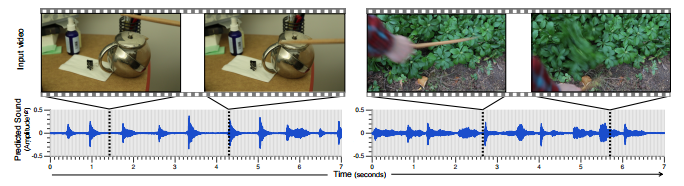
\includegraphics[width=0.8\textwidth]{figures/sonido}
		\caption{Ejemplo adición de sonidos a películas mudas. Imagen obtenida de~\cite{2015arXiv151208512O}.}
	\end{center}
\end{figure}


Además de las aplicaciones explicadas anteriormente existen muchísimas otras que surgen de las propias inquietudes del ser humano: reconocimiento facial, videovigilancia, identificación de posiciones... Sin embargo, ninguna de ellas ha sido desarrollada por completo, dejando una gran vía de investigación sobre el tema.\\

Este trabajo se centrará en la clasificación y detección de imágenes estáticas o en movimiento. La diferencia entre ambas aplicaciones es que la detección permite identificar en una única imagen diferentes objetos, independientemente del tamaño y la posición en la que se encuentren, mientras que la clasificación identifica una imagen entrante a la red como perteneciente a una clase determinada.\\

Por último, para implementar lo explicado anteriormente existen múltiples plataformas que facilitan el entrenamiento y la implementación de estas redes. TensorFlow, Keras, Theano, Caffe, Lassagne o Torch son algunos de los ejemplos más conocidos de estas plataformas. En este trabajo se utilizará la plataforma Caffe, una de las más veteranas. La elección de esta plataforma radica en el gran número de modelos pre-entrenados que proporciona la misma para poder implementar en las aplicaciones ahorrando tiempo al nuevo desarrollador. Además está centrado en la \acrshort{va}, lugar hacia el que se enfoca este trabajo, y, en caso de querer entrenar una nuevo red, resulta bastante rápido.\\


\section{Objetivos} \label{sec.objetivos}
Una vez contextualizado en trabajo, el objetivo general es claro: se pretende ahondar en el mundo de la \acrshort{ia}, en concreto en técnicas de Aprendizaje Profundo y \acrshort{cnn}, para obtener resultados que puedan resultar interesantes y desarrollar una aplicación que permita implementar estas técnicas con la mayor exactitud posible. Este objetivo general ha sido  articulado en varios subobjetivos concretos: 

\begin{itemize}
	\item \textbf{Estudio de la plataforma Caffe.} Se pretende estudiar la plataforma escogida para un correcto uso de la misma y la obtención de las redes que sean necesarias.
	\item \textbf{Desarrollo de componente que permita la clasificación de dígitos}, integrando una red entrenada con Caffe en el mismo.
	\item \textbf{Desarrollo de un banco de pruebas}, que permita agilizar la obtención de parámetros de evaluación de las distintas redes entrenadas.
	\item \textbf{Estudio y mejora de redes neuronales para la clasificación de dígitos.} Se realizarán diversas pruebas para tratar de alcanzar la red más robusta posible y utilizarla en el componente desarrollado.
	\item \textbf{Primera aproximación a la detección de Caffe.} Se estudiará la detección \acrfull{ssd} con Caffe para estímulos interesantes para aplicaciones futuras como personas, coches, bicicletas o señales de tráfico.
\end{itemize}

En la Figura~\ref{fig.diagrama} se desglosa, por semanas, el tiempo que ha llevado cada una de las tareas para la consecución de los objetivos.

\begin{figure}[H]
	\begin{center}
		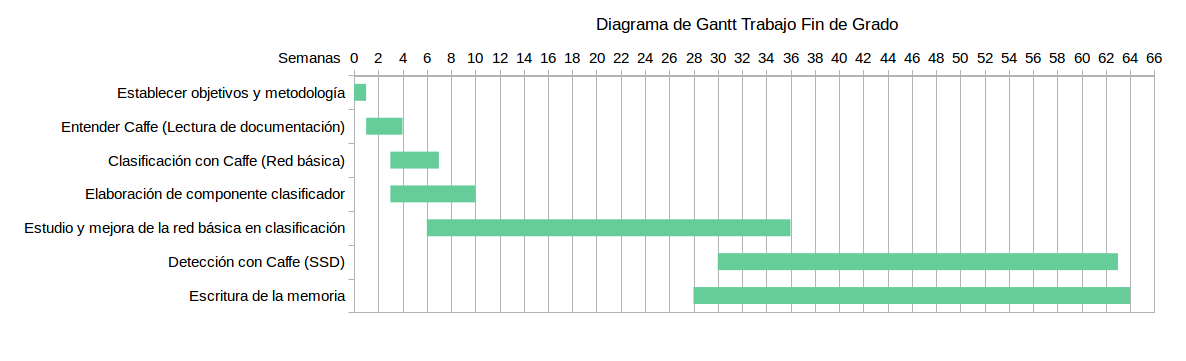
\includegraphics[width=1\textwidth]{figures/diagrama}
		\caption{Diagrama de Gantt del trabajo realizado.}
		\label{fig.diagrama}
	\end{center}
\end{figure}

\section{Metodología}
Para la consecución de los objetivos marcados se han utilizado varias herramientas que han permitido el seguimiento del trabajo por todos los miembros del grupo, permitiendo a todos ellos estar al tanto del trabajo realizado y aportar los comentarios o correcciones que se consideren necesarias.\\

Como herramienta principal, se establecieron reuniones semanales con todos los miembros del grupo, José María Cañas, Inmaculada Mora y David Pascual, que permitieron poner en común y discutir los resultados obtenidos y acordar las vías a seguir durante la siguiente semana.\\

Como herramientas complementarias, se utilizó una bitácora y un repositorio de Git Hub, que permitieron agilizar las reuniones al tener acceso de antemano al trabajo realizado. La bitácora se desarrolló empleando la \textit{Wiki} de JdeRobot\footnote{http://jderobot.org/Noyaga-tfg}, redactando cada semana el trabajo realizado y los resultados obtenidos. El repositorio de Git Hub\footnote{https://github.com/RoboticsURJC-students/2016-tfg-nuria-oyaga} permitió a todos los miembros del grupo acceder al código desarrollado, probarlo y establecer correcciones sobre el mismo.\\

El enfoque de desarrollo que se ha llevado a cabo es similiar al enfoque en espiral. Se establecen cuatro fases principales que son recorridas en forma de caracola. En primer lugar se marcaron los objetivos a alcanzar, seguido de una fase de análisis de riesgo para evaluar qué problemas era posible encontrarse al empezar el desarrollo. Tras evaluar las amenazas se procedió al propio desarrollo del trabajo y una última fase de evaluación del resultado obtenido. No existe un número fijo de iteraciones, produciéndose tantas como sean necesarias para obtener un resultado adecuado, incrementando en cada iteración el alcance del trabajo.

\section{Estructura de la memoria}
Para mostrar el trabajo realizado y los objetivos conseguidos se elabora la memoria con la estructura mostrada a continuación.\\

En el \textbf{Capítulo 1, Introducción y objetivos,} se sitúa el trabajo en el marco actual de la tecnología, la \acrshort{ia} y la sociedad en general. A continuación se establecen las metas que se pretenden alcanzar con el mismo.\\

El \textbf{Capítulo 2, Infraestructura,} describe todo el \textit{software} utilizado en el proyecto, incluyendo la principal plataforma, Caffe, y los conjuntos de datos empleados para la obtención y evaluación de las redes neuronales. Además, se explican los diferentes parámetros que serán empleados para evaluar las prestaciones de las redes creadas.\\

En el \textbf{Capítulo 3, Clasificación con Aprendizaje Profundo,} se expone todo el trabajo realizado para abordar el problema de la clasificación de dígitos con \acrshort{cnn}. En concreto, se describe el funcionamiento de Caffe en la clasificación, el componente creado, y las pruebas realizadas para conseguir una red robusta, con sus correspondientes resultados.\\

En el \textbf{Capítulo 4, Detección con Aprendizaje Profundo,}  se proporciona la información necesaria para realizar la detección con Caffe. Se muestran algunos resultados de pruebas preliminares, realizadas para una mejor comprensión del proceso de detección.\\

Por útlimo, el \textbf{Capítulo 5, Conclusiones y líneas futuras,} resume las conclusiones obtenidas en el trabajo y establece un posible plan de actuación futuro para continuar con la investigación en el tema que se aborda en el trabajo.

\lhead[]{CAPÍTULO \thechapter. OBJETIVOS}
\chapter{Objetivos}\label{cap.objetivos}
\lhead[]{CAPÍTULO \thechapter. INFRAESTRUCTURA}
\chapter{Infraestructura}\label{cap.infraestructura}
En este capítulo se expondrán los principales componentes software utilizados, centrados, principalmente, en la conexión con la cámara y el desarrollo, entrenamiento y test de la red neuronal. Además, se expone una descripción de las bases de datos de las que se partirá para realizar las distintas pruebas sobre la red neuronal. Estas bases de datos serán luego modificadas y adaptadas para el problema concreto que se plantee, permitiendo obtener diversas conclusiones acerca del comportamiento de la propia red y, así, emplear la más adecuada. Por último, serán expuestas los parámetros empleados para evaluar el impacto del aprendizaje en las redes neuronales y que permitirán escoger la red más adecuada para el problema.\\

\section{Software}

\subsection{JdeRobot}\label{sec.jderobot}
JdeRobot~\footnote{http://jderobot.org} es una plataforma de software libre que facilita la tarea de los desarrolladores en el campo de la robótica, visión por computador y otras relacionadas, siendo este su principal fin.\\ 

Está escrito en su mayoría en el lenguaje C ++ y proporciona un entorno de programación basado en componentes distribuidas, de tal manera que una aplicación está formada por una colección de varios componentes asincrónos y concurrentes. Esta estructura permite la ejecución de los distintos componentes en diferentes equipos, estableciendo una conexión entre ellos mediante el middleware de comunicaciones ICE. Además, se obtiene gran flexibiidad a la hora de desarrollar las aplicaciones, ya que estos componentes pueden escribirse en C ++, Python, Java, etc. y todos ellos interactúan a través de interfaces ICE explícitas.\\ 

A pesar de que esta plataforma incluye una gran variedad de herramientas y librerías para la programación de robots, y de una amplia gama de componentes previamente desarrollados para realizar tareas comunes en este ámbito, su uso no es la verdadera finalidad del proyecto, ya que únicamente se centrará en la utilización de uno de sus componentes para facilitar la obtención de las imágenes.
\vspace{10pt}
\begin{description}
\item[Camera Server] \hfill 
\vspace{10pt}
\\
Se trata de un componente que permite servir a un número determinado de cámaras, ya sean reales o simuladas, a partir de un archivo de vídeo. Internamente utiliza \textit{gstreamer} para el manejo y el procesamiento de las diferentes fuentes de vídeo.\\
\vspace{-10pt}
\\
Para su uso, es necesario editar su fichero de configuración, adaptándolo a las necesidades concretas que plantee la máquina. Dentro de este fichero se permite especificar los siguientes campos:\\
\vspace{-20pt}
\begin{itemize}
    \item Configuración de la red, donde se indica la dirección del servidor que va a recibir la petición.
    \item Número de cámaras que se servirán.
    \item Configuración de las cámaras. Se podrán modificar los siguientes campos para cada cámara:
    \begin{itemize}
         \item Nombre y breve descripción
         \item URI: string que define la fuente de vídeo
     	 \item Numerador y denominador del frame rate
         \item Altura y anchura de la imagen
         \item Formato de la imagen
         \item Invertir o no la imagen 
    \end{itemize}
\end{itemize}
\end{description}

\subsection{Caffe}\label{sec.caffe}
Caffe~\cite{jia2014caffe} es una plataforma de aprendizaje profundo que permite el desarrollo, entrenamiento y evaluación de redes neuronales. Incluye, además, modelos y ejemplos previamente trabajados para un mejor entendimiento de las redes neuronales. Es una plataforma de software libre, escrito en C ++, que utiliza la librería CUDA para el aprendizaje profundo y permite interfaces escritas en Python o Matlab.\\ 

Esta plataforma es interesante por múltiples factores. Además de incluir diferentes ejemplos y modelos ya entrenados, lo que ofrece mayor agilidad a la hora de empezar a entender el funcionamiento de las redes neuronales, es destacable la velocidad que ésta ofrece para el entrenamiento de las redes y su posterior evaluación, ya que está prevista con varios indicadores que permiten evaluar la propia red y compararla con otras.\\ 

Su base se encuentra en las redes neuronales convolucionales explicadas en el Capítulo \ref{cap.introduccion}, utilizando un entrenamiento por lotes. En concreto, su estructura y funcionamiento básico queda explicado en la Figura~\ref{fig.redCaffe}.\\

\begin{figure}[H]
	\begin{center}
		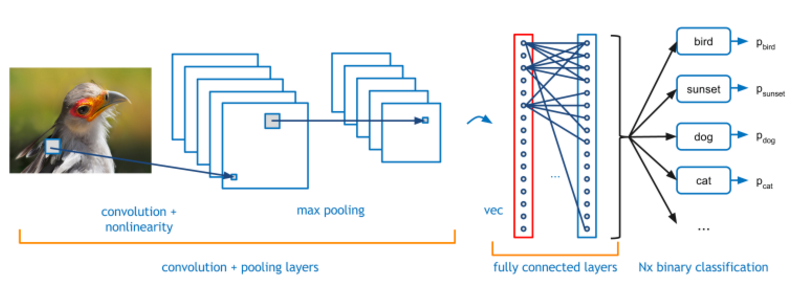
\includegraphics[width=0.6\textwidth]{figures/red_caffe}
		\caption{Estructura y funcionamiento básico de red en Caffe. Figura obtenida de~\cite{caffe}}
		\label{fig.redCaffe}
	\end{center}
\end{figure}

La plataforma utiliza una serie de capas (\textit{layers}), que, según su configuración y la distinta conexión entre ellas, permite la creación de diferentes redes neuronales. Estas capas se dividen en varios grupos, en función del tipo de entrada, el tipo de salida o la función que realiza cada una de ellas. Este trabajo no utiliza todas las capas existentes en la plataforma, a continuación se explicarán cada una de las capas empleadas, clasificadas según al grupo que pertenecen.
\vspace{20pt}
\begin{description}
\item[\textit{Data Layers}] \hfill 
\vspace{10pt}
\\
	Su uso se centra en la introducción de datos a la red neuronal, y estarán situadas siempre en la parte inferior de la misma. Estos datos provienen de diferentes vías que pueden ser: bases de datos eficientes como LMDB, utilizada en este trabajo, diréctamente desde la memoria o desde archivos en disco en HDF5 o formatos de imagen comunes.\\
	\vspace{-10pt}
	\\
	Dentro de esta capa es posible, además de especificar la ruta de los datos y el tamaño del lote (\textit{batch}), indicar la fase en la que se utilizarán los datos, entrenamiento o evaluación, así como algunos parámetros de transformación para el preprocesamiento de la imagen. En concreto, en este trabajo, se utilizarán datos de entrada para ambas fases y un factor de escala para establecer el rango de las imágenes en [0,1].
	\vspace{15pt}
	
\item[\textit{Vision Layers}] \hfill 
\vspace{10pt}
\\
	Este tipo de capas, típicamente toman una imagen de entrada y producen otra de salida, de forma que, aplicando una operación particular a alguna región de la entrada, se obtiene la región correspondiente de la salida. Caffe dispone de varias capas de este estilo, a continuación se comentan las dos utilizadas en el trabajo.
	\vspace{10pt}
	\begin{description}
	\item[\textit{Convolution Layer}] \hfill 
	\vspace{5pt}
	\\
		Realiza la convolución de la imagen de entrada con un conjunto de filtros de aprendizaje, cada uno produciendo un mapa de características en la imagen de salida. Se deben especificar datos como el número de salidas, el tamaño del filtro, el desplazamiento entre cada paso del filtro, y la inicialización y relleno de los pesos y \textit{bias}.
		\vspace{10pt}
	\item[\textit{Pooling Layer}] \hfill 
	\vspace{5pt}
	\\
		Combina la imagen de entrada aplicando una operación dentro de las regiones definidas por el filtro, siendo su finalidad la reducción del muestreo. Se especifican parámetros como el tipo de pooling a realizar, máximo, promedio o estocástico, el tamaño del filtro o el desplazamiento entre cada paso del filtro.
	\end{description}

\item[\textit{Common Layers}] \hfill
	\begin{description}
	\item[\textit{Inner Product}] \hfill 
	\vspace{5pt}
	\\
	Calcula un producto escalar con un conjunto de pesos aprendidos, y, de manera opcional, añade sesgos. Trata la entrada como un simple vector y produce una salida en forma de otro, estableciendo la altura y el ancho de cada \textit{bolb} en 1. Se establece el número de salidas, y la inicialización y relleno de los pesos y \textit{bias}.
	\vspace{10pt}
	\item[\textit{Dropout}] \hfill 
	\vspace{5pt}
	\\
	Durante el entrenamiento, únicamente, establece una porción aleatoria del conjunto de entrada a 0, ajustando el resto de la magnitud del vector en consecuencia, evistando así el sobre ajuste. Se debe indicar el ratio en un valor del 0 a 1, que indicará el porcentaje de muestras que se ignorarán.
	\end{description}

\vspace{15pt}	
\item[\textit{Activation / Neuron Layers}] \hfill  
\vspace{10pt}
\\
	En general estas capas son operadores de elementos que toman un \textit{bolb} inferior y producen uno superior del mismo tamaño. Existen varias capas con este funcionamiento en la plataforma, en concreto se empleará la \textit{\ac{ReLU}}.
	\vspace{10pt}
	\begin{description}
	\item[\textit{\ac{ReLU}}] \hfill  
	\vspace{5pt}
	\\
		Utiliza la función $y=max(0,x)$, cuya gráfica se define en la Figura~\ref{fig.reLu}, donde \textit{x} es la entrada a la neurona.
		\begin{figure}[H]
			\begin{center}
				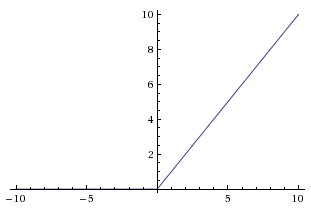
\includegraphics[width=0.5\textwidth]{figures/relu.jpeg}
				\caption{Función de activación \textit{\ac{ReLU}}.}
				\label{fig.reLu}
			\end{center}
		\end{figure} 
	\end{description}
	
\item[\textit{Loss Layers}] \hfill 
\vspace{10pt}
\\
	El cálculo de la pérdida permite el aprendizaje mediante la comparación de la salida con un objetivo y la asignación de un coste para minimizarla. Se calcula mediante el paso hacia adelante. Existen diferentes medidas de las que se destacan dos.
	\vspace{10pt}
	\begin{description}
	\item[\textit{Softmax with Loss}] \hfill 
	\vspace{5pt}
	\\
		La función \textit{softmax} se utiliza a menudo en la capa final de un clasificador basado en redes neuronales. Se trata de una función que modifica un vector K-dimensional de valores reales arbitrarios a un vector K-dimensional de valores reales en el rango (0, 1] que suman 1.\\
		\vspace{-10pt}
		\\
		Esta capa es conceptualmente idéntica a una capa de \textit{softmax}, la cual calcula la función con el mismo nombre, seguida por una capa de pérdida logística multinomial, proporcionando un gradiente numéricamente más estable.
		Se calcula l pérdida como: 
		$$E = \frac{-1}{N} \sum\limits_{n=1}^N \log(\hat{p}_{n,l_n})$$
		Siendo $N$ el número total de muestras, $\hat{p}$ las probabilidades de cada etiqueta para cada muestra y $l_n$ las etiquetas existentes. Se definen las etiquetas existentes como $l_n\in[0, 1, 2, ..., K-1]$, siendo $K$ el total de clases. Adicionalmente, se debe multiplicar todo por $-1$ ya que se aplica el logaritmo a una probabilidad, oscilante entre 0 y 1, obteniendo un resultado negativo, y el que se desea obtener debe ser positivo.
		\vspace{10pt}
	\item[Accuracy] \hfill 
	\vspace{5pt}
	\\
		Esta capa calcula únicamente la tasa de acierto de la red, es decir, el número de aciertos en la clasificación referenciado al número total de muestras analizadas.
		Se calcula como:
		$$\frac{1}{N} \sum\limits_{n=1}^N \delta\{ \hat{l}_n = l_n \}$$

		Donde $\hat{l_n}$ es la etiqueta que la red decide en la clasificación y, al igual que en el caso anterior, $N$  es el número total de muestras y $l_n$ las etiquetas existentes. Por último, la función $\delta\{x\}$ se define como:
		$$\delta\{ \textup{condición}\} = \left\{ \begin{array}{lr} 1 &  \textup{si condición} \\ 0 & \mbox{resto} \end{array} \right.$$
	\end{description}
	
\end{description}
\vspace{10pt}

Por último, además de las capas y parámetros definidos anteriormente, Caffe, permite el desarrollo de un solucionador (\textit{solver}) en el que se podrán ajustar parámetros como el número de iteraciones totales que se ejecutarán, el de evaluación que se van a realizar, cada cuantas iteraciones se realizará esa evaluación, o se sacarán redes intermedias.\\

Para Caffe, el número de iteraciones no se corresponde con el número de veces que la red recorre la base de datos al completo, sino como las veces que se pasa por cada lote al completo. Esto viene dado porque, debido a la amplia dimensión de las bases de datos necesarias para desarrollar el aprendzaje profundo, según se explicación en el Capítulo~\ref{cap.introduccion}, será necesaria una división de la misma en pequeños lotes para que ordenador no se bloquee en el tratamiento de las mismas. De esta manera, se define el número de épocas, es decir, el número de veces que se recorre de manera completa la base de datos, con la siguiente expresión:\\
$$\textup{N.Epocas}=\frac{\textup{Tamaño lote de entrenamiento}\times \textup{Total iteraciones}}{\textup{Muestras entrenamiento}} $$\\

\subsection{DroidCam}\label{sec.droid}
DroidCam~\footnote{https://www.dev47apps.com/} es una aplicación que permite convertir un dispositivo móvil en una cámara web, estableciendo una conexión mediante WiFi/LAN, modo servidor wifi, o USB. Esta aplicación es muy usada para establecer videoconferencias a través de plataformas como Skype o Google+, entre otras aplicaciones. En este trabajo será usada para obtener el flujo de vídeo desde un dispositivo distinto a la webcam del ordenador, haciendo más sencillo el manejo del mismo.\\

La aplicación funciona con un componente cliente en el ordenador que instala los controladores de la cámara web y conecta el equipo con el dispositivo Android, que deberá tener instalada la misma aplicación.\\

Entre sus características principales destacan:
	\begin{itemize}
		\item Incluye sonido e imagen
		\item Conexión por diferentes medios
		\item Uso de otras apliaciones con DroidCam en segundo plano
		\item Cámara IP de vigilancia con acceso MJPEG
	\end{itemize}

\vspace{10pt}
\section{Bases de datos}

\subsection{MNIST}\label{sec.minst}
La base de datos \textit{\ac{MNIST}}~\footnote{http://yann.lecun.com/exdb/mnist/} está formada por diferentes imágenes con números escritos a mano y consta de un conjunto de entrenamiento de 60.000 ejemplos y otro de prueba de 10.000 ejemplos. Es una buena base de datos para personas que quieren probar técnicas de aprendizaje y métodos de reconocimiento de patrones en datos del mundo real, mientras que dedican un mínimo esfuerzo a preprocesar y formatear. \\

Se trata de un subconjunto de una más grande, \textit{\ac{NIST}}, en la que las imágenes originales en blanco y negro fueron normalizadas en el tamaño para encajar en un cuadro de 20x20 píxeles, preservando su relación de aspecto. Las imágenes obtenidas contienen niveles de gris como resultado de la técnica anti-aliasing utilizada por el algoritmo de normalización. Estas imágenes se centraron en una de 28x28 calculando el centro de masa de los píxeles y trasladando la imagen para situar este punto en el centro del campo 28x28.\\

Fue construida a partir de la Base de Datos Especial 3 y la Base de Datos Especial 1 del \ac{NIST}, que contienen imágenes binarias de dígitos manuscritos. \ac{NIST} originalmente designó SD-3 como su conjunto de entrenamiento y SD-1 como su conjunto de pruebas. Sin embargo, SD-3 es mucho más limpio y más fácil de reconocer que SD-1.Esto es debido a que SD-3 fue recogido entre los empleados de la Oficina del Censo, mientras que el SD-1 fue recogido entre los estudiantes de secundaria. Dado que para una buena extracción de conclusiones es necesario que el resultado sea independiente de la elección del conjunto de entrenamiento y de prueba entre el conjunto completo de muestras, fue necesaria la elaboración de un nuevo conjunto en el que ambas bases de datos estuviesen representadas de manera equitativa. Además, se aseguraron de que los conjuntos de escritores en el de entrenamiento y el de prueba son disjuntos.\\

\subsection{COCO}
Microsoft \textit{\ac{COCO}}~\footnote{http://mscoco.org/} es un gran conjunto de datos de imágenes diseñado para la detección de objetos, segmentación y generación de subtítulos~\cite{veit2016cocotext}. Alguna de las características principales de este conjunto de datos son:
	\begin{itemize}
         \item Múltiples objetos en cada imagen
     	 \item Más de 300.000 imágenes
         \item Más de 2 millones de instancias
         \item 80 categorías de objetos
    \end{itemize}
    
Esta plataforma se ha desarrollado para varios retos, en concreto es de interés el reto de la detección, establecido en 2016. Se utilizan conjuntos de entrenamiento, prueba y validación con sus correspondientes anotaciones. \ac{COCO} tiene tres tipos de anotaciones: instancias de objeto, puntos clave de objeto y leyendas de imagen, que se almacenan utilizando el formato de archivo \textit{\ac{JSON}} y comparten estructura de datos establecida en la Figura~\ref{fig.basicStruc}. \\

\begin{figure}[H]
	\begin{center}
		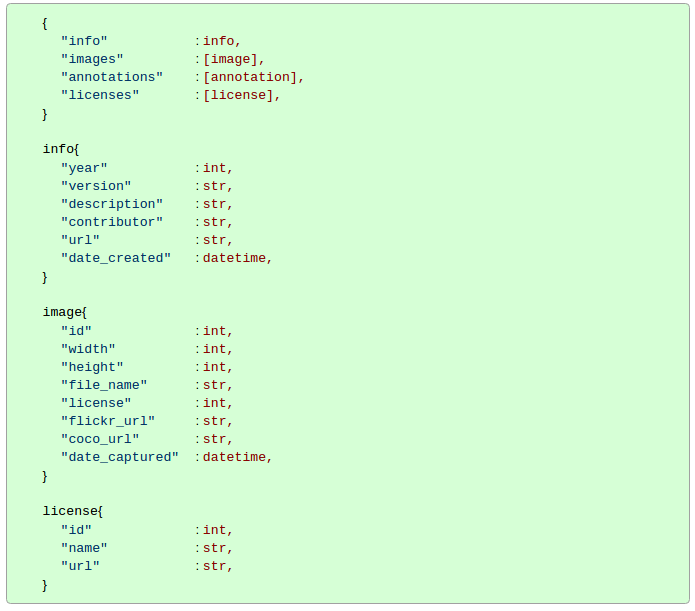
\includegraphics[width=0.8\textwidth]{figures/basic_structure_annotations.png}
		\caption{Estructura básica de anotaciones en \ac{COCO}.}
		\label{fig.basicStruc}
	\end{center}
\end{figure} 

Para la detección son de interés las anotaciones de instancias de objetos, cuya estructura se muestra en la Figura~\ref{fig.objInst}.Cada anotación de instancia contiene una serie de campos, incluyendo el ID de categoría y la máscara de segmentación del objeto. El formato de segmentación depende de si la instancia representa un único objeto (\textit{iscrowd}~=~0), en cuyo caso se utilizan polígonos, o una colección de objetos (\textit{iscrowd}~=~1), en cuyo caso se utiliza \textit{\ac{RLE}}. Debe tenerse en cuenta que un único objeto puede requerir múltiples polígonos, y que las anotaciones de la multitud se utilizan para etiquetar grandes grupos de objetos. Además, se proporciona una caja delimitadora para cada objeto, cuyas coordenadas se miden desde la esquina superior izquierda de la imagen y están indexadas en 0. Finalmente, el campo de categorías  almacena el mapeo del ID de categoría a los nombres de categoría y supercategoría.

\begin{figure}[H]
	\begin{center}
		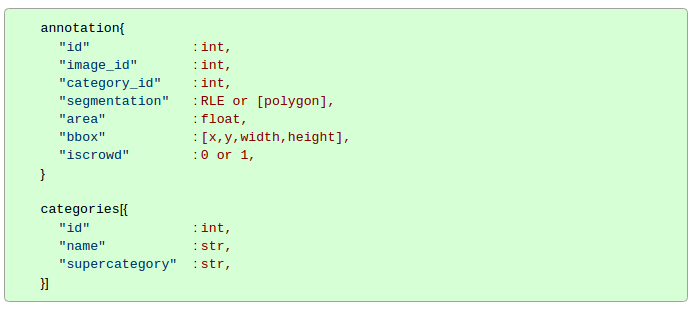
\includegraphics[width=0.8\textwidth]{figures/instancia_objetos.png}
		\caption{Estructura de instancias de objetos en \ac{COCO}.}
		\label{fig.objInst}
	\end{center}
\end{figure}

\subsection{VOC}
El objetivo del desafío de \textit{\ac{VOC}} \cite{Everingham10} es investigar el desempeño de los métodos de reconocimiento en un amplio espectro de imágenes naturales. Para ello, se requiere que los conjuntos de datos \ac{VOC} contengan variabilidad significativa en términos de tamaño del objeto, orientación, pose, iluminación, posición y oclusión. También es importante que los conjuntos de datos no muestren sesgos sistemáticos, por ejemplo, favoreciendo imágenes con objetos centrados o una buena iluminación. Del mismo modo, para garantizar un entrenamiento y una evaluación precisa, es necesario que las anotaciones de imagen sean consistentes, precisas y exhaustivas para las clases especificadas.\\

Teniendo claros estos conceptos, en 2007, se llevó a cabo una recolección de imágenes, como las mostradas en la Figura~\ref{fig.voc_example}, formando el conjunto de datos \textit{\ac{VOC}}\textit{2007}~\cite{pascal-voc-2007}. Este conjunto dispone de dos grandes bases de datos, una de ellas compuesta por un conjunto de validación y otro de entrenamiento, y la otra con un único conjunto de test. Ambas bases de datos contienen alrededor de 5000 imágenes en las que se representan, apróximadamente, 12.000 objetos diferentes, por lo que, en total, este conjunto dispone de unas 10000 imágenes en las que se reperesentan unos 24000 objetos. En el año 2012 se modifica este conjunto, aumentando a 11530 el número de imágenes con representación de 27450 objetos diferentes~\cite{pascal-voc-2012}.

\begin{figure}[H]
	\begin{center}
		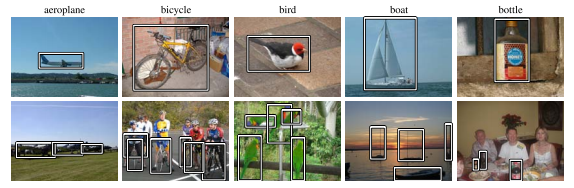
\includegraphics[width=0.7\textwidth]{figures/vocexample}
		\caption{Ejemplos de imágenes en \ac{VOC}. Imagen tomada de~\cite{Everingham10}}.
		\label{fig.voc_example}
	\end{center}
\end{figure}

Dado que la finalidad de este conjunto de datos es permitir el desarrollo tanto de la clasificación de objetos como la detección de los mismos, será necesario que estas imágenes contengan una serie de anotaciones. Entre otras cosas, estas anotaciones contienen dos atributos importantes para ambas tareas:

\begin{itemize}
	\item Para la \textbf{clasificación}, se debe indicar la clase de objeto que es. Los objetos de este conjunto estan clasificados en 20 clases diferentes. En la Figura~\ref{fig.clasesVOC} se puede observar la división que se hace de cada una de las clases y las distintas clases existentes.
	\item Para la \textbf{detección}, será necesario indicar, para cada objeto, la \textit{bounding box}. Se trata de un cuadro delimitador alineado con el eje que rodea la extensión del objeto visible en la imagen, permitiendo identificar el objeto en la imagen.
\end{itemize}
\begin{figure}[H]
	\begin{center}
		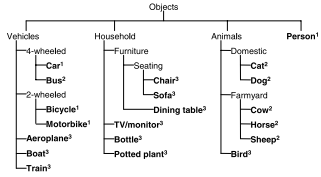
\includegraphics[width=0.7\textwidth]{figures/vocclasses}
		\caption{Estructura de las clases en \ac{VOC}2007. Imagen tomada de~\cite{Everingham10}}. El año de inclusión de cada clase en el desafío está indicado por
		superíndices: $2005^1$, $2006^2$, $2007^3$.
		\label{fig.clasesVOC}
	\end{center}
\end{figure}

\section{Evaluación de prestaciones} \label{sec.prestaciones}
Existen multitud de parámetros que permiten la evaluación de las redes neuronales, sin embargo, en este proyecto, todas las comparaciones se centrarán en cinco de ellas: \textit{accuracy}, \textit{loss}, matriz de confusión, \textit{precision} y \textit{recall}~\cite{pullum2007guidance}.\\

Las dos primeras fueron explicadas en la Sección~\ref{sec.caffe}, por lo que no se ahondará más sobre ellas. Las tres restantes serán explicdas más profundamente, y de manera totalmente teórica a continuación.

\subsection{Matriz de confusión}
Una matriz de confusión (Kohavi y Provost, 1998) contiene información sobre las clasificaciones reales y predichas hechas por un sistema de clasificación. El rendimiento de estos sistemas se evalúa comúnmente utilizando los datos de la matriz~\cite{metrics}. En la Figura~\ref{fig.matriz} se muestra un ejemplo sencillo de la construcción de esta matriz donde:
\begin{itemize}
	\item \textbf{\textit{a}} es el número de predicciones correctas de que una instancia es negativa
	\item \textbf{\textit{b}} es el número de predicciones incorrectas de que una instancia es positiva
	\item \textbf{\textit{c}} es el número de predicciones incorrectas de una instancia negativa
	\item \textbf{\textit{d}} es el número de predicciones correctas de que una instancia es positiva.
\end{itemize}

\begin{figure}[H]
	\begin{center}
		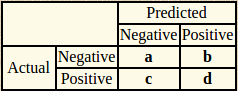
\includegraphics[width=0.3\textwidth]{figures/matrizexample}
		\caption{Ejemplo sencillo de matriz de confusión. Imagen tomada de~\cite{metrics}}.
		\label{fig.matriz}
	\end{center}
\end{figure}

Además de ayudar con el cálculo de \textit{precision} y \textit{recall}, es importante mirar la matriz de confusión para analizar sus resultados, ya que también proporciona información importante sobre dónde el clasificador funciona mal~\cite{metrics2}. Para que una matriz proporcione información sobre el correcto funcionamiento de un clasificador se obtendrán valores altos en la diagonal, y lo más pequeños posible en el resto de celdas de la misma.

\subsection{\textit{Precision}}
Se trata de la proporción de los casos positivos predichos que fueron correctos~\cite{metrics}. Para obtener este valor en el ejemplo sencillo anteriormente explicado se utiliza la fórmula:
$$P = \frac{d}{b+d} $$
Donde $P$ es el valor de \textit{precision} y $b$ y $d$ los mismo valores explicados en la sección anterior.\\

En un caso más complejo en el que la clasificación no sea binaria, se deben de tener en cuenta todas las clases, por ello la fórmula queda expresada de la siguiente forma~\cite{metrics2}:
$$P = \frac{TP_X}{TP_X + FP_X} $$
Donde:
\begin{itemize}
	\item $TP_X$ se corresponde el número de verdaderos positivos para la clase $X$, es decir, el valor de aciertos correspondiente para dicha clase, situado en la diagonal.
	\item $FP_X$ se corresponde el número de falsos positivos para la clase $X$, es decir, el número de veces que se predijo dicha clase sin haber sido producida, correspondiente con la suma del resto de celdas en la misma fila.
\end{itemize}

\subsection{\textit{Recall}}
Se trata de la proporción de casos positivos que fueron correctamente identificados~\cite{metrics}. Para el ejemplo sencillo se calcula mediante la siguiente expresión:
$$R = \frac{d}{c+d} $$
Donde $R$ es el valor de \textit{recall} y $c$ y $d$ los mismo valores explicados anteriormente.\\

Al igual que en el caso de la sección anterior, en caso de tener una clasificación multiclase se deberás tener en cuenta todas ellas, utilizando para ello la expresión~\cite{metrics2}:
$$R = \frac{TP_X}{TP_X +FN_X} $$
Donde $TP_X$ se corresponde con lo explicado en la sección anterior y $FN_X$ se corresponde con los falsos negativos para la clase $X$, es decir, el número de veces que se predijo errónamente otra clase habiéndose producido $X$, correspondiente con la suma del resto de la columna. 
\lhead[]{CAPÍTULO \thechapter. DESARROLLO}
\chapter{Desarrollo}\label{cap.desarrollo}
En este capítulo se expondrá el trabajo realizado para el entendimiento del problema de clasificación, elaborando un amplio estudio sobre las variantes posibles sobre las redes entrenadas, y una primera aproximación a la detección,todo ello con redes neuronales desarrolladas sobre la plataforma Caffe.\\
\section{Clasificador de dígitos}
Para el estudio de la clasificación empleando redes neuronales desarrolladas con Caffe, se optó por la transformación, según determinados criterios, de la red básica proporcionada por la propia plataforma en este ámbito.\\
\subsection{Red básica}
Esta red está orientada a la clasificación de números utilizando en el entrenamiento la base de datos numérica MNIST, explicada en el Capítulo~\ref{cap.infraestructura}. Para su entrenamiento, Caffe proporciona tres archivos que se deberán editar para adaptar la red al problema que se abarque.\\
\begin{description}
	\item[Definición de la red] \hfill \\
	Caffe utiliza el archivo 
	\textit{lenet\_train\_test.prototxt} para la especificación de todos los parámetros que son necesarios en el entrenamiento de la red, es decir, define las imágenes que se emplearán, la propia estructura de la red y la forma en la que se analizarán las imágenes proporcionadas, todo ello empleando diferentes capas (\textit{layers}).\\
	
	La primera línea de este documento es utilizada para indicar el nombre que se le quiere dar a la red.
	\vspace{5pt}
	\begin{lstlisting}[frame=single]
	name: "LeNet"
	\end{lstlisting}
	
	En concreto, esta red recibe el nombre de LeNet, un tipo de red que es conocida por un buen funcionamiento en las tareas de clasificiación de dígitos y que, por lo general, consta de una capa convolucional seguida por una capa de agrupamiento (\textit{pooling}), repetido dos veces y, finalmente, dos capas totalmente conectadas similares a las perceptrones multicapa convencionales. En el ejemplo de Caffe, la estructura habitual de la red LeNet se ve ligeramente modificada, ya que en lugar de emplear una función de activacion sigmoidal se utiliza una linear.\\
	
	Tras la definición del nombre se definen dos capas de datos, una de ellas correspondiente a los datos de entrenamiento de la red y, la otra, correspondiente a los datos que se utilizarán para realizar el test durante el entrenamiento para obtener datos de \textit{accuracy} y \textit{loss}.
	\vspace{5pt}
	\begin{lstlisting}[frame=single]
	layer {
		name: "mnist"
		type: "Data"
		top: "data"
		top: "label"
		include {phase: TRAIN}
		transform_param {scale: 0.00390625}
		data_param {
			source: "examples/mnist/mnist_train_lmdb"
			batch_size: 64
			backend: LMDB
		}
	}
	\end{lstlisting}
	
	Es importante que los parámetros de transformación, en este caso un factor de escala que establece el rango de la imagen en [0,1], sean los mismos en ambas fases, pues si se evaluase la red con una transformación de la imágen distinta a la aplicada en el entrenamiento los resultados obtenidos no serían reales.\\
	Se utilizará, por tanto, dos capas de datos que difieren en la fase en la que se utilizarán los datos, entrenamiento o evaluación de la red, el tamaño del lote, siendo 64 muestras para el entrenamiento y 100 para el test, y la ruta de la que se cogen los datos.\\
	
	A continuación, se comienzan a definir las capas del entrenamiento propiamente dicho. Se intercala una capa de convolución con una de agrupamiento y se repite dos veces.
	\vspace{5pt}
	\begin{lstlisting}[frame=single]
	layer {
		name: "conv1"
		type: "Convolution"
		bottom: "data"
		top: "conv1"
		param {lr_mult: 1}
		param {lr_mult: 2}
		convolution_param {
			num_output: 20
			kernel_size: 5
			stride: 1
			weight_filler {type: "xavier"}
			bias_filler {type: "constant"}
		}
	}	
	\end{lstlisting}
	
	En la capa de convolución, explicada en el Capítulo~\ref{cap.infraestructura}, se define que el tamaño del filtro será de 5x5 y que se obtendrán 20 salidas, en la segunda capa de convolución, sin embargo, se obtendrán 50 salidas. Además se define el algoritmo "Xavier" para la inicialización de los pesos, que determina automáticamente la escala de inicialización basada en el número de entradas y de las neuronas de salida, y la inicialización del \textit{bias} mediante una constante que por defecto es 0.
	\vspace{5pt}
	\begin{lstlisting}[frame=single]
	layer {
		name: "pool1"
		type: "Pooling"
		bottom: "conv1"
		top: "pool1"
		pooling_param {
			pool: MAX
			kernel_size: 2
			stride: 2
		}
	}	
	\end{lstlisting}
	
	La capa de agrupamiento, también explicada en el Capítulo~\ref{cap.infraestructura}, será alimentada por la capa de convolución anterior y alimentará a la siguiente en caso de que la haya. Se definen en ella un tamaño de filtro de 2x2, un intervalo de dos muestras entre cada aplicación del filtro, por lo que no hay solape, y el método del máximo para realizar el agrupamiento.

	
	\item[Definición del solucionador] \hfill 
	\vspace{10pt}
	\\
	
	\item[Ejecución de la red] \hfill 
	\vspace{10pt}
	\\
		
\end{description}


\lhead[]{CAPÍTULO \thechapter. EXPERIMENTOS}
\include{5-Experimentos}
\lhead[]{CAPÍTULO \thechapter. CONCLUSIONES}
\chapter{Conclusiones y líneas futuras}\label{cap.conclusiones}
Por último, en este capítulo se exponen las conclusiones alcanzadas con el desarrollo del trabajo, así como posibles líneas para continuar en el futuro, ayudándose de los resultados obtenidos en el desarrollo del mismo.

\section{Conclusiones}
El desarrollo de este trabajo ha permitido establecer una serie de conclusiones en el ámbito de aprendizaje profundo mediante el empleo de redes neuronales entrenadas con Caffe. A pesar de que el desarrollo del trabajo tenía como objetivos establecer conclusiones sobre las dos tareas principales de esta técnica, clasificación y detección, por las propias características del trabajo únicamente se obtuvieron conclusiones firmes sobre la clasificación, dejando abierta la puerta a una futura investigación en el problema de la detección con estas redes. A continuación se exponen todas las conclusiones que fueron establecidas gracias a la obtención de distintos resultados por la evaluación de las redes neuronales entrenadas.

\begin{itemize}
	\item La plataforma Caffe posee un funcionamiento muy adecuado para el ámbito de la visión artificial gracias a un entrenamiento rápido y a gran número de ejemplos y facilidades para el mismo. Además proporcionan la posibilidad de entrenamiento de redes tanto para clasificación como detección.
	\item Las redes neuronales con Caffe pueden ser entrenadas con diferentes conjuntos de datos, siempre en formato \acrshort{lmdb}, obteniendo resultados muy diferentes en función de la composición de las mismas. 
	\item Para el ejemplo tratado con la base de datos \acrshort{mnist} para la clasificación de dígitos, al variar la composición de estas bases de datos, se han obtenido diversas conclusiones interesantes que han permitido mejorar de forma considerable la red final entrenada.
	\begin{itemize}
		\item El entrenamiento con imágenes de borde amplia el número aciertos en la clasificación, pues independiza la misma del fondo de la imagen.
		\item Al incluir imágenes con transformaciones en en entrenamiento de la red, la precisión de la clasificación aumenta, permitiendo obtener una red más robusta.
		\item La precisión obtenida al incluir un alto número de imágenes transformadas frente a la que se obtiene disminuyendo ese número de imágenes es muy similar, por lo que no es necesario incluir un gran número de estas imágenes en el entrenamiento.
		\item Sobre la inclusión de la imagen limpia en el entrenamiento, siendo ésta la imagen sin ninguna transformación, se obtienen resultados que avalan que no es necesario incluirla para obtener una mayor precisión.
	\end{itemize}
	\item Se ha elaborado un componente bastante y robusto con Python que permite la clasificación de dígitos mostrados a una cámara RGB gracias a una red entrenada con Caffe gracias a las conclusiones obtenidas en el punto anterior.
\end{itemize}

Como se mencionó anteriormente, los resultados obtenidos en los exprerimentos de la detección no son concluyenetes, por lo que no es posible establecer conclusiones firmes sobre esta técnica.

\section{Líneas futuras}
Para seguir con la investigación abordada en este trabajo se pueden seguir dos claras tendencias marcadas por los dos grande problemas que se pueden abordar, detección y clasificación.
\begin{itemize}
	\item Por un lado, el que no se haya obtenido resultados concluyentes en el campo de la detección permite continuar en futuras investigaciones en esta línea, tratando de obtener una red robusta para esta tarea mediante la modificación de la red entrenada con diferentes bases de datos o estructuras de red.
	\item Por otro lado, en el campo de la clasificación, es posible extender lo aprendido para un ejemplo sencillo, la clasificación de dígitos con redes neuronales gracias al conjunto de datos \acrshort{mnist}, a un ejemplo más complejo como puede ser la clasificación de signos o de señales de tráfico.
\end{itemize}

Finalmente, la aplicación ideal consiste en una mezcla de ambos problemas. De esta manera, por ejemplo, sería posible la elaboración de una aplicación que permitiese a un choche circular de forma autónoma, detectando los estímulos que recibe de la carretera y clasificando los mismos para actuar en consecuencia a la clase detectada.\\

Éstos son solo algunos ejemplos de los diferentes problemas que se pueden tratar de abordar con esta tecnología. La cantidad de tareas que se pueden tratar de realizar es tan amplia como el número de problemas que se le pueden presentar a un ser humano en su día a día, pues la finalidad de estas aplicaciones no es otra que facilitar la vida diaria de las personas.

%%%%%%%%%%%%%%% Bibliograí­a %%%%%%%%%%%%%%%
\lhead[]{BIBLIOGRAFÍA}
\addcontentsline{toc}{chapter}{Bibliografía}
\bibliographystyle{unsrt}
\bibliography{Memoria}

\end{document}